\chapter{光电倍增管的性能测试与筛选}
\label{ch:pmt_test}
由于制造工艺的限制,光电倍增管具有很强的个体差异性,即不同管子的性能差异较大。
因此,在光电倍增管大规模应用时,往往要求对每支管子进行详细的测试,以得到它们各自的性能参数信息。
利用这些信息,探测器的研制者可以淘汰性能参数不达标的管子,可以决定管子在探测器整体中的安装位置,可以得到管子的额定工作电压,甚至可以在探测器部署运行后调节其实际工作电压,最终使探测器整体的探测性能达到最佳。

对于PSD所使用的R4443型光电倍增管,Hamamatsu公司对每支出厂的管子进行了基本性能的测试(包括阳极暗电流、长时间稳定性、阴极/阳极的光灵敏度以及阴极/阳极的蓝光灵敏度),并提供了相应的测试结果。
然而,这些测试只对一个工作电压点进行,而且使用的测试条件(连续、强烈的白炽光照射)与R4443在PSD中的实际工作条件(低强度、低频率的脉冲光照射)迥异。
另外,PSD使用双打拿极引出的分压器电路与上述出厂测试使用的标准分压器差别较大,导致R4443的工作状态也不一致。
因此,这些信息只能定性地给出各支管子的基本性能,不能作为PSD研制过程的定量参考。

上述因素决定了我们需要根据PSD的具体需求,在实验室独立对R4443光电倍增管进行性能参数测试。
为此,我们专门设计并搭建了一套的PMT批量测试平台。
本章首先对该测试平台进行了介绍,并详细叙述了该平台在R4443光电倍增管的性能测试中的应用。
之后过程以及结果。
根据

\section{PSD对光电倍增管的测试需求}

\section{PMT批量测试平台}
\label{sec:pmt_test:testbench}
\emph{为什么需要特质的批量测试平台}

\subsection{功能与特点}

\begin{figure}[htb]
	\centering
	\includegraphics[width=\textwidth]{chap/pmt_test/fig/testbench_schematic.eps}
	\caption{PMT批量测试平台的原理框图}
	\label{fig:pmt_test:testbench_schematic}
\end{figure}

\subsection{硬件结构与组成}
% 总述硬件结构,之后依次介绍各组件以及相关测试结果。

% 主体平台
\begin{figure}[htbp]
	\centering
	\subfloat[][铝合金暗箱]{
		\label{fig:pmt_test:blackbox}
		\includegraphics[width=0.49\textwidth]{chap/pmt_test/fig/black_box.jpg}
	}
	\subfloat[][三维移动平台与固定平台]{
		\label{fig:pmt_test:stages}
		\includegraphics[width=0.49\textwidth]{chap/pmt_test/fig/stages.jpg}
	}
	\caption{PMT批量测试平台的主体结构}
	\label{fig:blindfigure}
\end{figure}

% 紧固件
\begin{figure}[htbp]
	\centering
	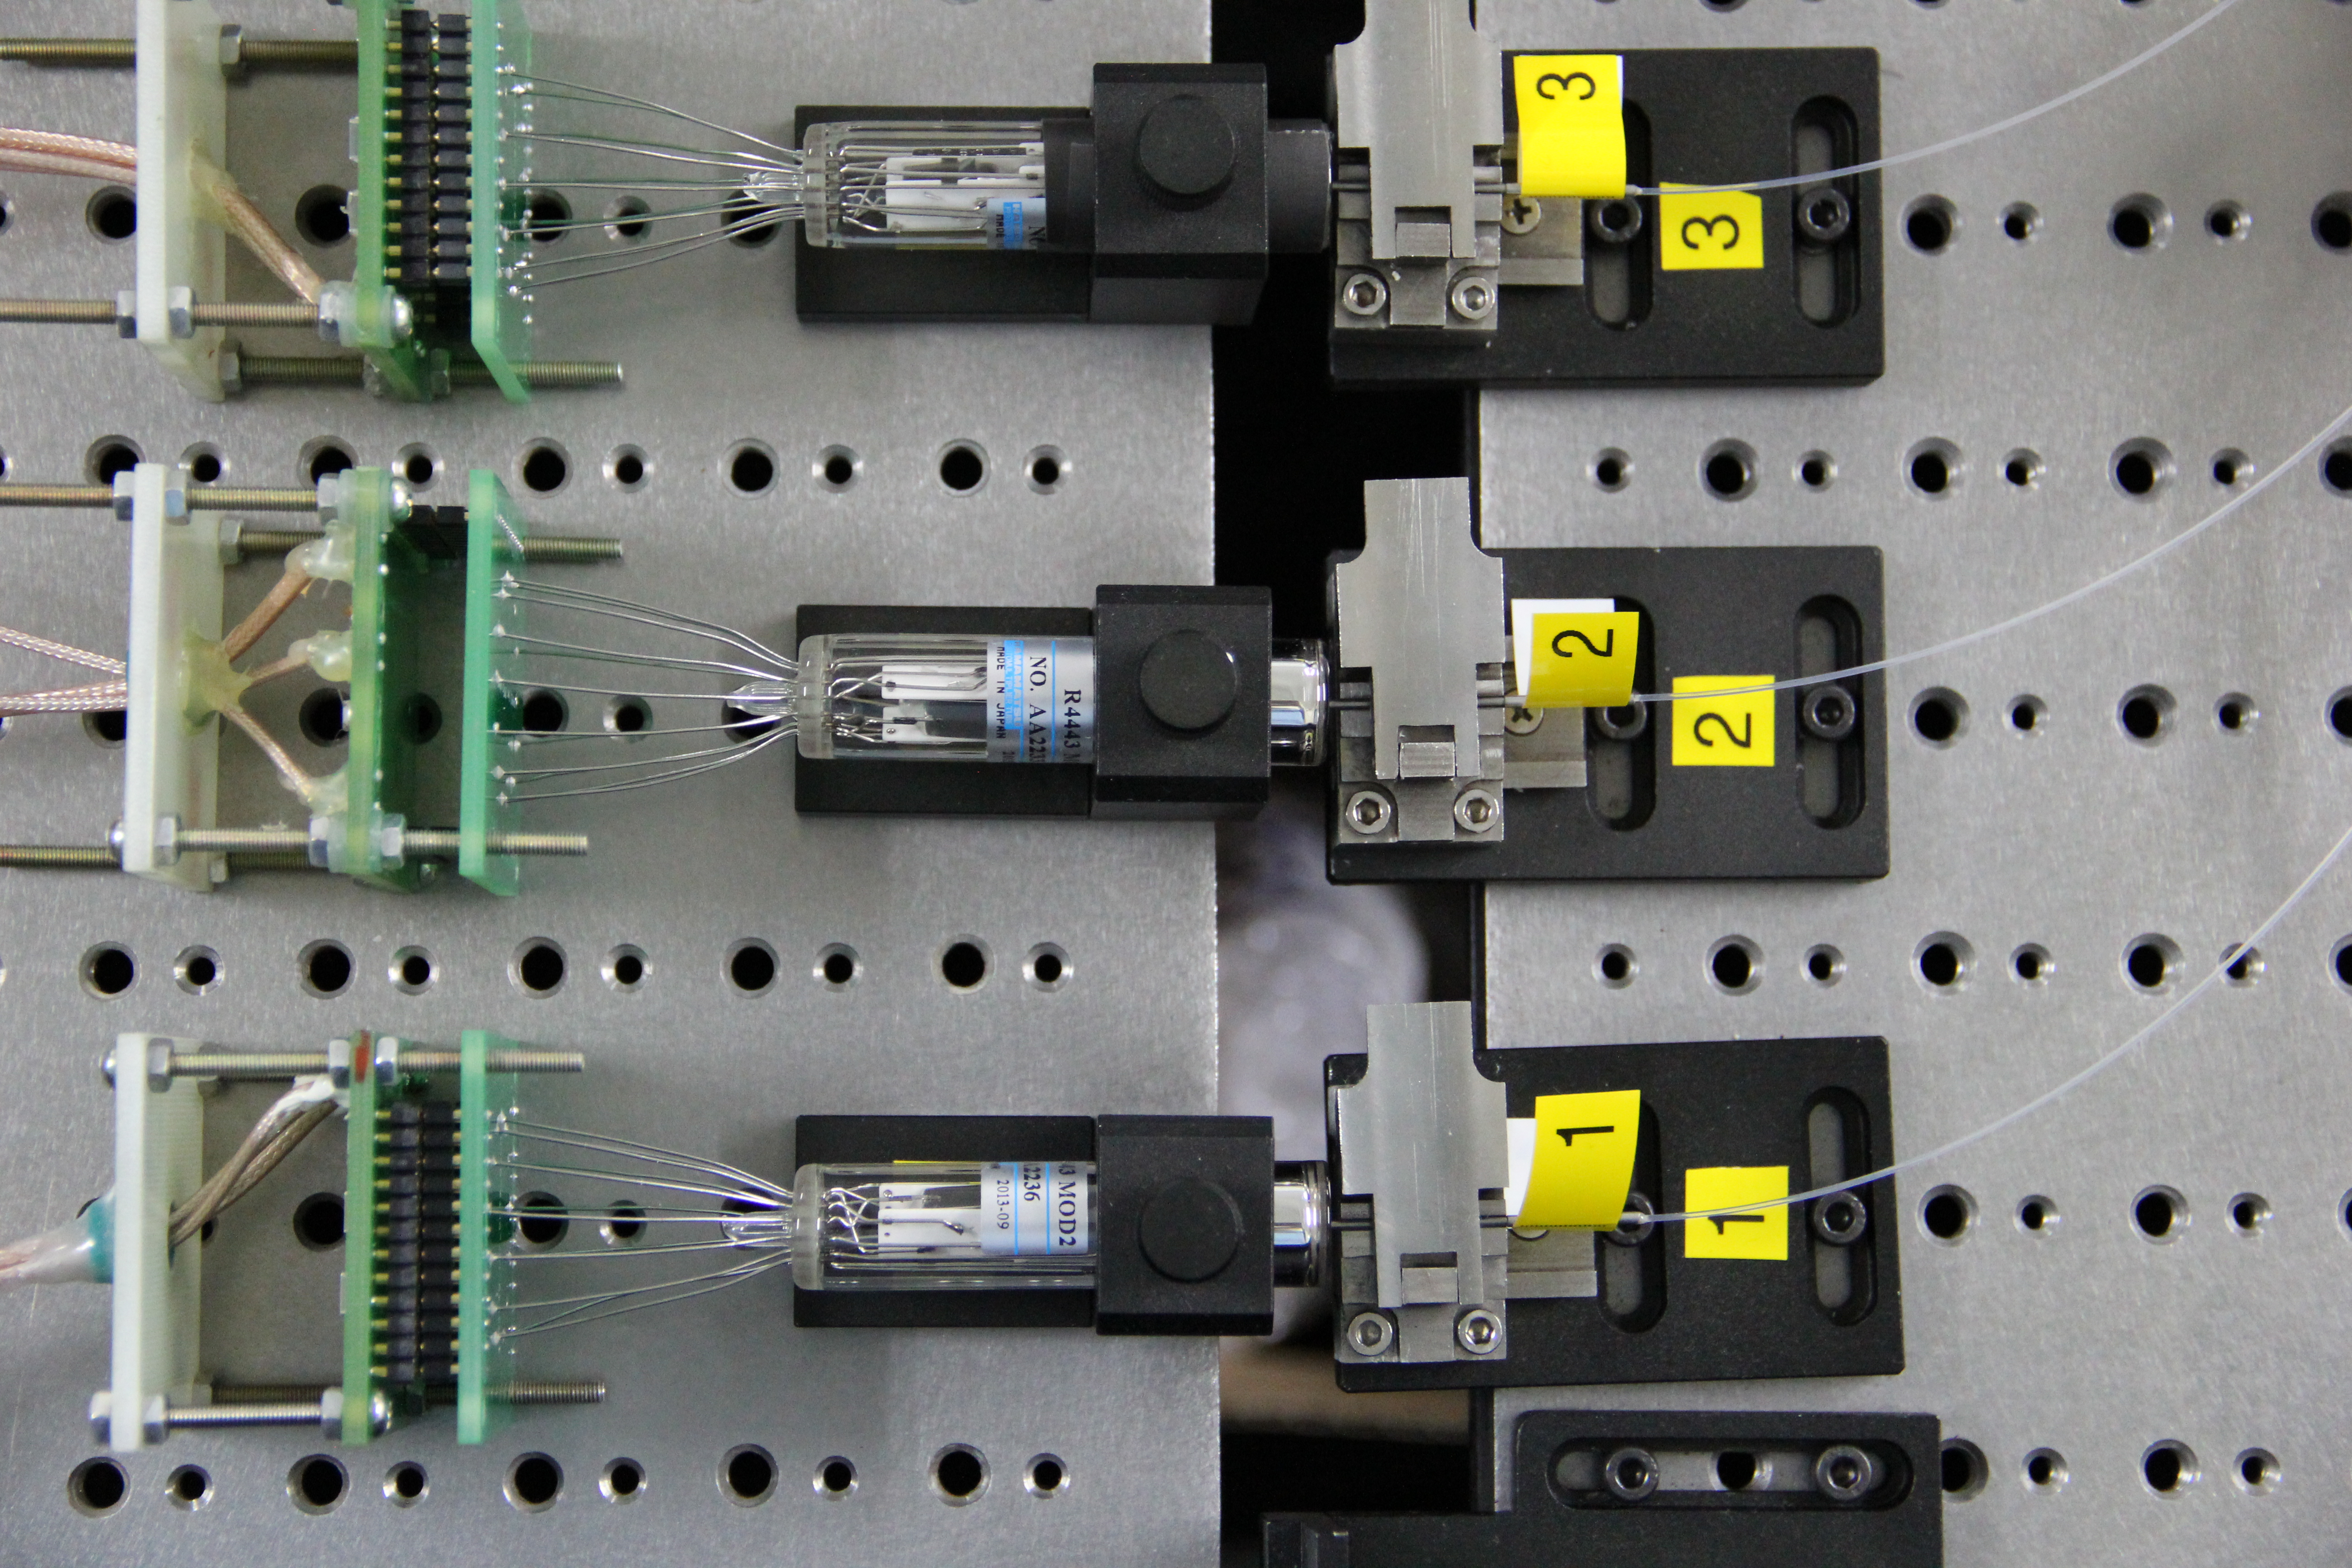
\includegraphics[width=0.6\textwidth]{chap/pmt_test/fig/fixtures.jpg}
	\caption{PMT紧固件和光纤紧固件}
	\label{fig:pmt_test:fixtures}
\end{figure}

% 光源
\begin{figure}[htbp]
	\centering
	\subfloat[][1)LED 2)积分球 3)集束光纤]{
		\label{fig:pmt_test:lightsource_components}
		\includegraphics[width=0.49\textwidth]{chap/pmt_test/fig/lightsource_components.jpg}
	}
	\subfloat[][各组件耦合在一起]{
		\label{fig:pmt_test:lightsource_integration}
		\includegraphics[width=0.49\textwidth]{chap/pmt_test/fig/lightsource_integration.jpg}
	}		
	\caption{PMT批量测试平台的光分配系统}
	\label{fig:pmt_test:light_distribution}
\end{figure}

\begin{figure}[htbp]
	\centering
	\includegraphics[width=0.65\textwidth]{chap/pmt_test/fig/integrationsphere_uniformity.eps}
	\caption{\SI{5}{cm}铝合金积分球输出端口的光均匀性}
	\label{fig:pmt_test:integrationsphere_uniformity}
\end{figure}

% 光源驱动器
\begin{figure}[htbp]
	\centering
	\includegraphics[width=0.65\textwidth]{chap/pmt_test/fig/led_pulse.jpg}
	\caption{输入方波脉冲驱动的LED光得到的R4443原始波形}
	\label{fig:pmt_test:led_pulse}
\end{figure}

\begin{figure}[htbp]
	\centering
	\includegraphics[width=0.62\textwidth]{chap/pmt_test/fig/led_response.eps}
	\caption{LED输出脉冲的光强度与AFG3253脉冲幅度的非线性关系}
	\label{fig:pmt_test:led_response}
\end{figure}

% 集束光纤
\begin{figure}[htbp]
	\centering
	\includegraphics[width=0.7\textwidth]{chap/pmt_test/fig/fiber_difference.eps}
	\caption{集束光纤各通道的光传输差异性}
	\label{fig:pmt_test:fiber_difference}
\end{figure}

\subsection{测控软件}
% 最好这里做一个归纳性的介绍,具体细节设计放到附录中


\section{R4443裸管的性能测试}

\subsection{相对增益的测量}
\subsection{Dynode8/Dynode5增益比值的测量}
\subsection{光阴极均匀性}
\subsection{PMT批量测试平台的长期稳定性}

\section{PMT的筛选}
\subsection{筛选方案}
工厂参数。
\subsection{参考单元模块的MIPs响应}
\subsection{与塑闪单元条的匹配}